\documentclass[sn-apa]{sn-jnl} % APA Reference Style 

\usepackage{graphicx}
\usepackage{amsmath,amssymb}
\usepackage[style=apa]{biblatex}
\addbibresource{my_bib.bib}

\begin{document}

\title[Supplementary Materials]{Supplementary Materials}

\maketitle

\section{Supplementary Note on Modality and Replication}

A recurring question in replication research is how to interpret differences
that result from pragmatic adaptations rather than intentional design choices.
In Ge et al. (2021), data were collected in two laboratories using different
hardware (Tobii TX300 in Hong Kong; EyeLink 1000 in the Netherlands). These
systems differ in sampling rate, calibration routines, and testing environments,
yet both sites were part of the same original study. This illustrates that even
within a single project, cross-site variability in equipment and context is
common. As \textcite{mcmanus2024} notes, replication studies will always involve
some deviations, and the critical requirement is that they are reported
transparently rather than ignored or over-interpreted as new methodological
conditions.

Our study followed this principle. We used web-based eye-tracking with
WebGazer.js and online recruitment via Prolific because these were the feasible
tools for collecting data. We did not design this as a test of “online versus
lab” methods, but as a pragmatic adaptation that allowed replication with
available resources. Web-based eye-tracking introduces limitations in temporal
precision relative to Tobii or EyeLink systems, but it also brings important
advantages: scalability, access to broader participant pools, and consistency
across testing sites. These trade-offs are consistent with broader open science
standards \parencite{goodman2016reproducibility} and with recent
field-specific guidelines for eye-tracking \parencite{godfroid2025reporting}. Moreover,
a growing body of research demonstrates that online eye-tracking is a viable
method for visual world studies when combined with careful calibration and
exclusion criteria \parencite[e.g.,][]{AOW}. 

A further point is that population differences almost always entail laboratory
differences. To study learners in different countries or speakers of different
languages, researchers must recruit across sites, each with its own hardware,
software, and testing conditions. Thus, methodological heterogeneity is
unavoidable when addressing cross-linguistic questions. The critical issue is
not whether every site, tool, or modality is identical, but whether the design
is faithfully reproduced and reported in sufficient detail for evaluation
\parencite{mcmanus2024}. Following prior work on online VWP experiments,
including \textcite{AOW}, our study demonstrates that replication can
preserve design fidelity while adapting pragmatically to new platforms. In this
sense, the move online should be understood as a practical decision, not a theoretical manipulation, and one that is consistent with the broader reality of replication in applied linguistics and psycholinguistics.


\section{Supplemental Materials: Frame Rate Distribution}

\noindent
Supplemental Materials Figure 1 shows the distribution of effective frame rates across participants. Data were collected using 
WebGazer.js embedded in Gorilla, with participants’ own webcams. Because hardware could not be standardized (e.g., webcam model, screen size, or viewing 
distance), we instead report observable sampling characteristics. The shaded grey region marks the 5~Hz cutoff used for exclusion. Individual points (black) 
represent trial-level frame rates, red points show mean frame rate per participant, and the blue line indicates the overall mean across participants. This visualization illustrates that, while variability is inherent in online testing, most participants recorded above the cutoff and contributed usable data.

\begin{figure}[h]
    \centering
    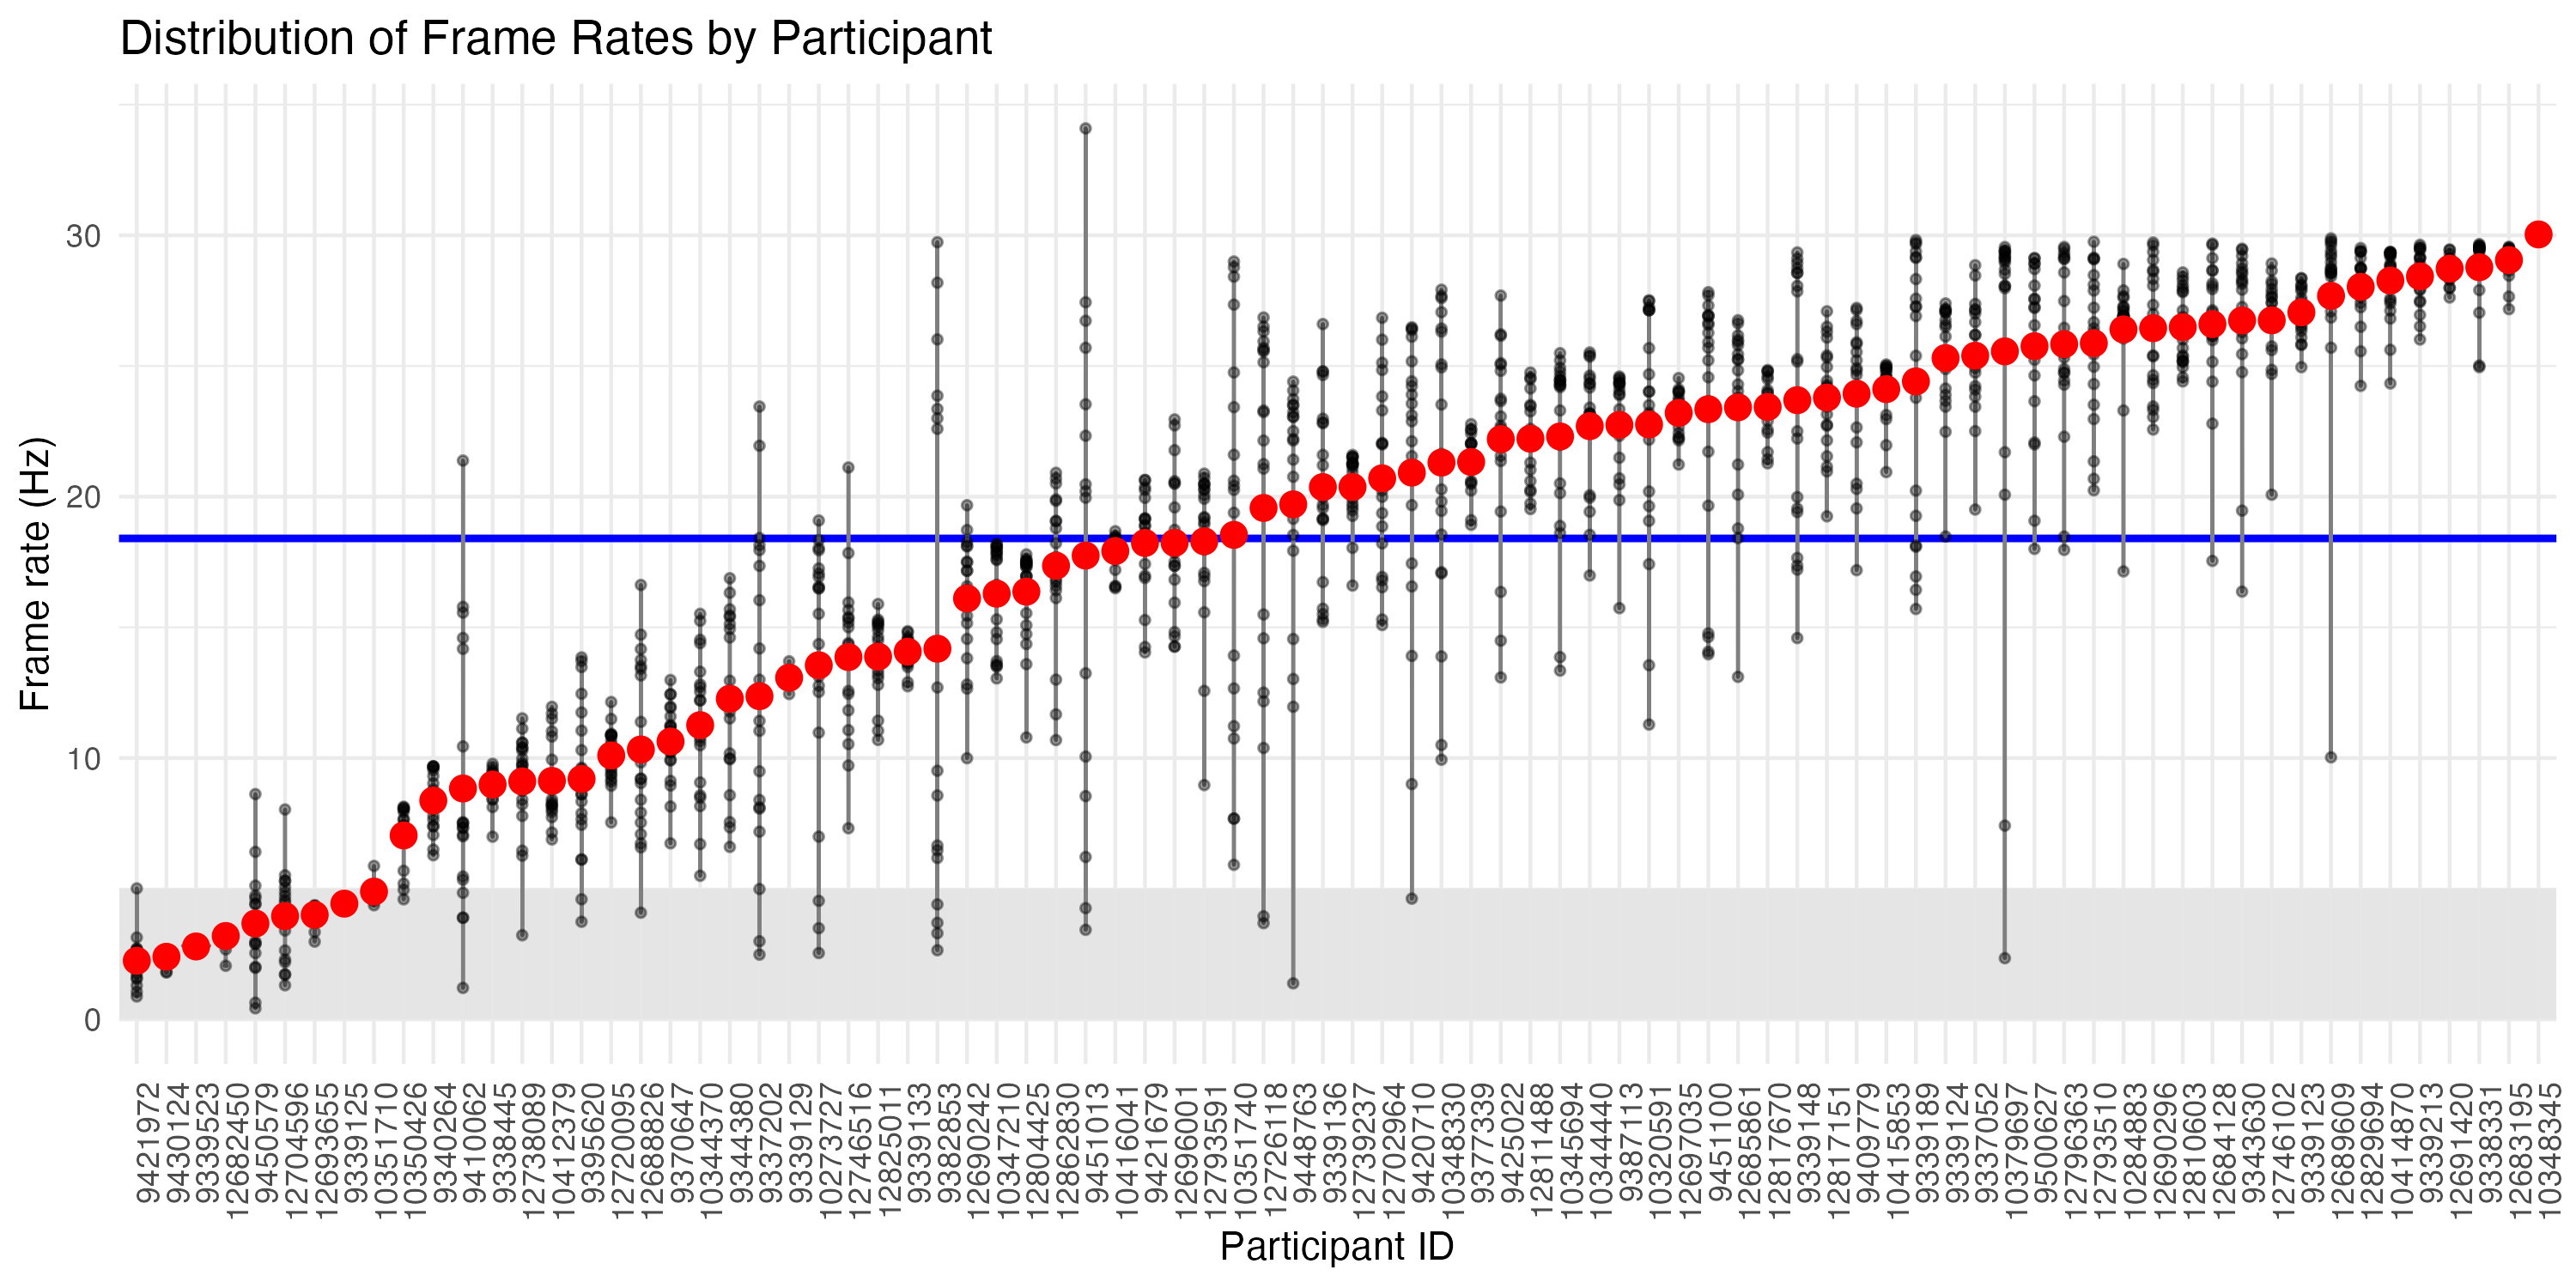
\includegraphics[width=\textwidth]{viz/fr.png}
    \caption{Distribution of effective frame rates across participants. Grey 
    shading marks the 5~Hz cutoff used for exclusion. Black points represent 
    trial-level frame rates, red points indicate participant means, and the 
    blue line shows the overall mean.}
    \label{fig:frame_rate}
\end{figure}

This style figure was inspired by-  \textcite{AOW}. 

\end{document}
